\documentclass[border=10pt]{standalone}
\usepackage{tikz}
\usepackage{xcolor}
\usepackage{mathpazo}
\usetikzlibrary{shapes.geometric, arrows, shadows, positioning, fit, backgrounds, decorations.pathreplacing, shapes.multipart}

% Define custom colors for DevTrack
\definecolor{devtrackblue}{RGB}{41, 128, 185}
\definecolor{devtrackdarkblue}{RGB}{44, 62, 80}
\definecolor{devtrackgreen}{RGB}{46, 204, 113}
\definecolor{devtrackorange}{RGB}{230, 126, 34}
\definecolor{devtrackred}{RGB}{231, 76, 60}
\definecolor{devtrackgray}{RGB}{149, 165, 166}
\definecolor{devtrackbg}{RGB}{236, 240, 241}

\begin{document}

%%%%%%%%%%%%%%%%%%%%%%%%%%%%%%%%%%%%%%%%%
% Platform Banner
%%%%%%%%%%%%%%%%%%%%%%%%%%%%%%%%%%%%%%%%%
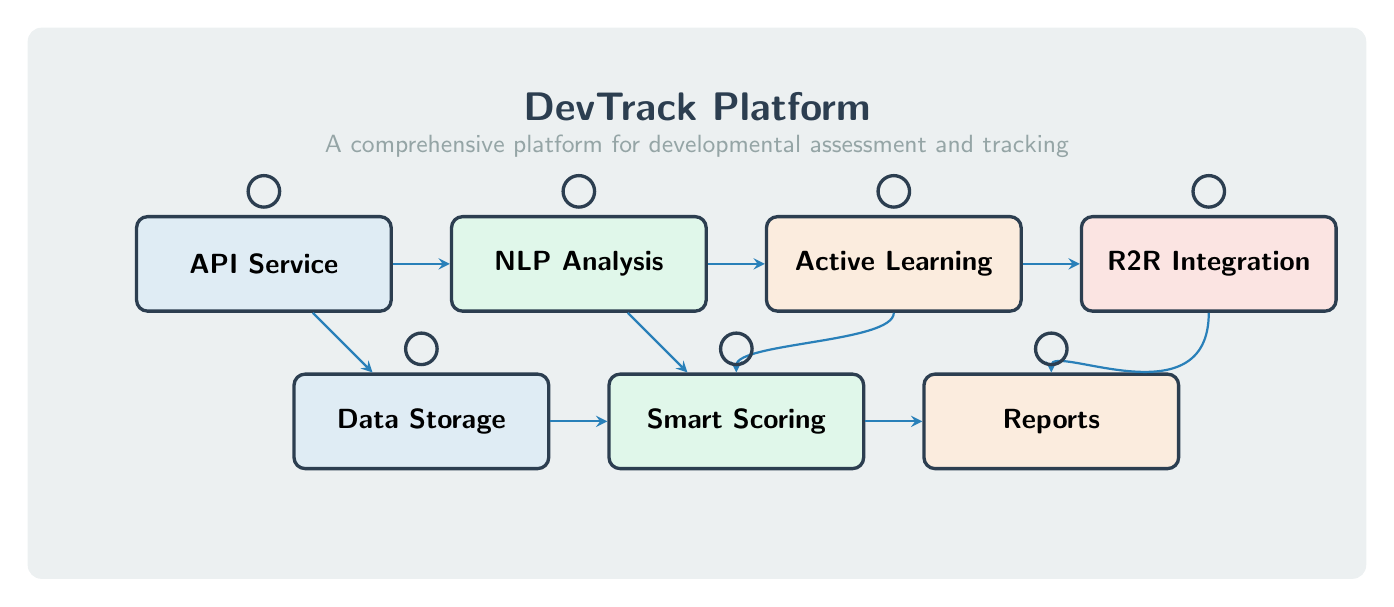
\begin{tikzpicture}[
    node distance=1.5cm,
    box/.style={
        rectangle,
        rounded corners,
        draw=devtrackdarkblue,
        fill=white,
        very thick,
        text width=2.5cm,
        minimum height=1.2cm,
        text centered,
        font=\sffamily\bfseries
    },
    arrow/.style={
        ->,
        >=stealth,
        thick,
        devtrackblue
    },
    title/.style={
        font=\sffamily\bfseries\Large,
        text=devtrackdarkblue
    },
    subtitle/.style={
        font=\sffamily\small,
        text=devtrackgray
    }
]

% Background rectangle
\fill[devtrackbg, rounded corners=5pt] (-1,-1) rectangle (16,6);

% Title
\node[title] at (7.5,5) {DevTrack Platform};
\node[subtitle] at (7.5,4.5) {A comprehensive platform for developmental assessment and tracking};

% Platform components
\node[box, fill=devtrackblue!15, text width=3cm] (api) at (2,3) {API Service};
\node[box, fill=devtrackgreen!15, text width=3cm] (nlp) at (6,3) {NLP Analysis};
\node[box, fill=devtrackorange!15, text width=3cm] (active) at (10,3) {Active Learning};
\node[box, fill=devtrackred!15, text width=3cm] (r2r) at (14,3) {R2R Integration};

\node[box, fill=devtrackblue!15, text width=3cm] (data) at (4,1) {Data Storage};
\node[box, fill=devtrackgreen!15, text width=3cm] (scoring) at (8,1) {Smart Scoring};
\node[box, fill=devtrackorange!15, text width=3cm] (report) at (12,1) {Reports};

% Connections
\draw[arrow] (api) -- (nlp);
\draw[arrow] (nlp) -- (active);
\draw[arrow] (active) -- (r2r);
\draw[arrow] (api) -- (data);
\draw[arrow] (data) -- (scoring);
\draw[arrow] (scoring) -- (report);
\draw[arrow] (nlp) -- (scoring);
\draw[arrow] (active) .. controls +(down:1) and +(up:1) .. (scoring);
\draw[arrow] (r2r) .. controls +(down:2) and +(up:1) .. (report);

% Icons (represented by simple shapes)
\foreach \pos in {api, nlp, active, r2r, data, scoring, report} {
    \draw[devtrackdarkblue, very thick] (\pos.north) + (0,0.3) circle (0.2);
}

\end{tikzpicture}

%%%%%%%%%%%%%%%%%%%%%%%%%%%%%%%%%%%%%%%%%
% Scoring Pipeline Diagram
%%%%%%%%%%%%%%%%%%%%%%%%%%%%%%%%%%%%%%%%%
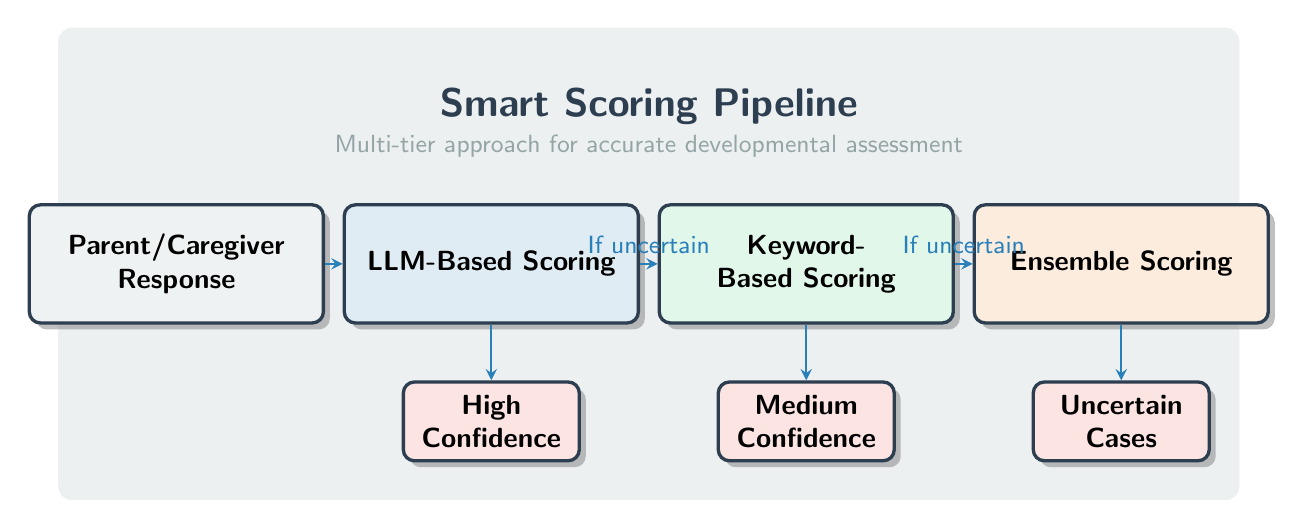
\begin{tikzpicture}[
    node distance=2cm,
    block/.style={
        rectangle,
        rounded corners,
        draw=devtrackdarkblue,
        fill=white,
        very thick,
        text width=3.5cm,
        minimum height=1.5cm,
        text centered,
        font=\sffamily\bfseries,
        drop shadow
    },
    arrow/.style={
        ->,
        >=stealth,
        thick,
        devtrackblue
    },
    title/.style={
        font=\sffamily\bfseries\Large,
        text=devtrackdarkblue
    },
    subtitle/.style={
        font=\sffamily\small,
        text=devtrackgray
    }
]

% Background rectangle
\fill[devtrackbg, rounded corners=5pt] (-0.5,-1) rectangle (14.5,5);

% Title
\node[title] at (7,4) {Smart Scoring Pipeline};
\node[subtitle] at (7,3.5) {Multi-tier approach for accurate developmental assessment};

% Input
\node[block, fill=devtrackgray!15] (input) at (1,2) {Parent/Caregiver Response};

% Primary Scoring
\node[block, fill=devtrackblue!15] (llm) at (5,2) {LLM-Based Scoring};

% Secondary Scoring
\node[block, fill=devtrackgreen!15] (keyword) at (9,2) {Keyword-Based Scoring};

% Tertiary/Ensemble Scoring
\node[block, fill=devtrackorange!15] (ensemble) at (13,2) {Ensemble Scoring};

% Confidence Indicators
\node[block, fill=devtrackred!15, text width=2cm, minimum height=1cm] (high) at (5,0) {High Confidence};
\node[block, fill=devtrackred!15, text width=2cm, minimum height=1cm] (medium) at (9,0) {Medium Confidence};
\node[block, fill=devtrackred!15, text width=2cm, minimum height=1cm] (low) at (13,0) {Uncertain Cases};

% Arrows
\draw[arrow] (input) -- (llm);
\draw[arrow] (llm) -- (keyword) node[midway, above, font=\sffamily\small] {If uncertain};
\draw[arrow] (keyword) -- (ensemble) node[midway, above, font=\sffamily\small] {If uncertain};
\draw[arrow] (llm) -- (high);
\draw[arrow] (keyword) -- (medium);
\draw[arrow] (ensemble) -- (low);

\end{tikzpicture}

%%%%%%%%%%%%%%%%%%%%%%%%%%%%%%%%%%%%%%%%%
% Test Results Dashboard - FIXED VERSION
%%%%%%%%%%%%%%%%%%%%%%%%%%%%%%%%%%%%%%%%%
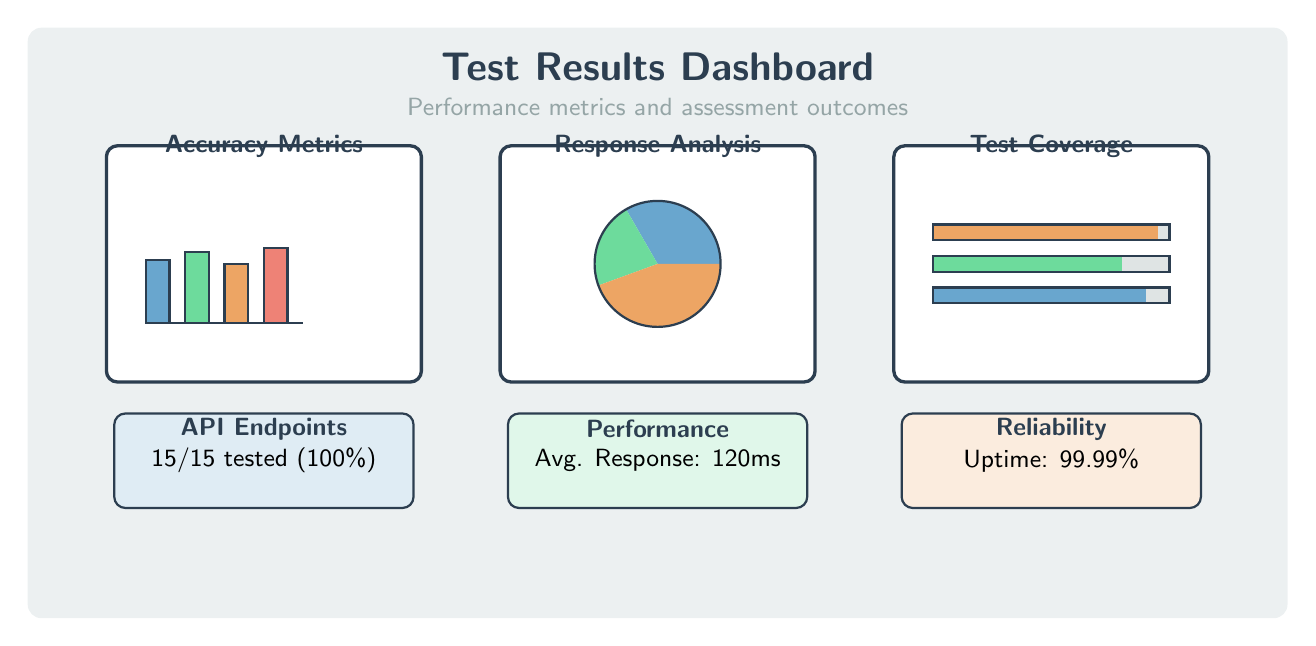
\begin{tikzpicture}[
    node distance=1.5cm,
    title/.style={
        font=\sffamily\bfseries\Large,
        text=devtrackdarkblue
    },
    subtitle/.style={
        font=\sffamily\small,
        text=devtrackgray
    },
    panel/.style={
        rectangle,
        rounded corners,
        draw=devtrackdarkblue,
        very thick,
        fill=white,
        minimum width=4cm,
        minimum height=3cm
    },
    smallpanel/.style={
        rectangle,
        rounded corners,
        draw=devtrackdarkblue,
        thick,
        fill=white,
        minimum width=3.8cm,
        minimum height=1.2cm
    },
    mylabel/.style={
        font=\sffamily\bfseries\small,
        text=devtrackdarkblue
    }
]

% Background rectangle
\fill[devtrackbg, rounded corners=5pt] (-0.5,-0.5) rectangle (15.5,7);

% Title
\node[title] at (7.5,6.5) {Test Results Dashboard};
\node[subtitle] at (7.5,6) {Performance metrics and assessment outcomes};

% Panels
\node[panel] (accuracy) at (2.5,4) {};
\node[panel] (response) at (7.5,4) {};
\node[panel] (coverage) at (12.5,4) {};

\node[mylabel] at (2.5,5.5) {Accuracy Metrics};
\node[mylabel] at (7.5,5.5) {Response Analysis};
\node[mylabel] at (12.5,5.5) {Test Coverage};

% Accuracy Chart (simple bar chart)
\begin{scope}[shift={(1,3.25)}]
    \foreach \x/\h/\c in {0/0.8/devtrackblue, 0.5/0.9/devtrackgreen, 1/0.75/devtrackorange, 1.5/0.95/devtrackred} {
        \fill[\c!70] (\x,0) rectangle (\x+0.3,\h);
        \draw[devtrackdarkblue, thick] (\x,0) rectangle (\x+0.3,\h);
    }
    \draw[devtrackdarkblue, thick] (0,0) -- (2,0);
\end{scope}

% Response Analysis (pie chart)
\begin{scope}[shift={(7.5,4)}]
    \fill[devtrackblue!70] (0,0) -- (0:0.8) arc (0:120:0.8) -- cycle;
    \fill[devtrackgreen!70] (0,0) -- (120:0.8) arc (120:200:0.8) -- cycle;
    \fill[devtrackorange!70] (0,0) -- (200:0.8) arc (200:360:0.8) -- cycle;
    \draw[devtrackdarkblue, thick] (0,0) circle (0.8);
\end{scope}

% Test Coverage (progress indicators)
\begin{scope}[shift={(11,3.5)}]
    \foreach \y/\w/\c in {0/0.9/devtrackblue, 0.4/0.8/devtrackgreen, 0.8/0.95/devtrackorange} {
        \fill[devtrackgray!30] (0,\y) rectangle (3,\y+0.2);
        \fill[\c!70] (0,\y) rectangle (3*\w,\y+0.2);
        \draw[devtrackdarkblue, thick] (0,\y) rectangle (3,\y+0.2);
    }
\end{scope}

% Bottom panels
\node[smallpanel, fill=devtrackblue!15] (api) at (2.5,1.5) {};
\node[smallpanel, fill=devtrackgreen!15] (performance) at (7.5,1.5) {};
\node[smallpanel, fill=devtrackorange!15] (reliability) at (12.5,1.5) {};

\node[mylabel] at (2.5,1.9) {API Endpoints};
\node[font=\sffamily\small] at (2.5,1.5) {15/15 tested (100\%)};

\node[mylabel] at (7.5,1.9) {Performance};
\node[font=\sffamily\small] at (7.5,1.5) {Avg. Response: 120ms};

\node[mylabel] at (12.5,1.9) {Reliability};
\node[font=\sffamily\small] at (12.5,1.5) {Uptime: 99.99\%};

\end{tikzpicture}

%%%%%%%%%%%%%%%%%%%%%%%%%%%%%%%%%%%%%%%%%
% Active Learning System
%%%%%%%%%%%%%%%%%%%%%%%%%%%%%%%%%%%%%%%%%
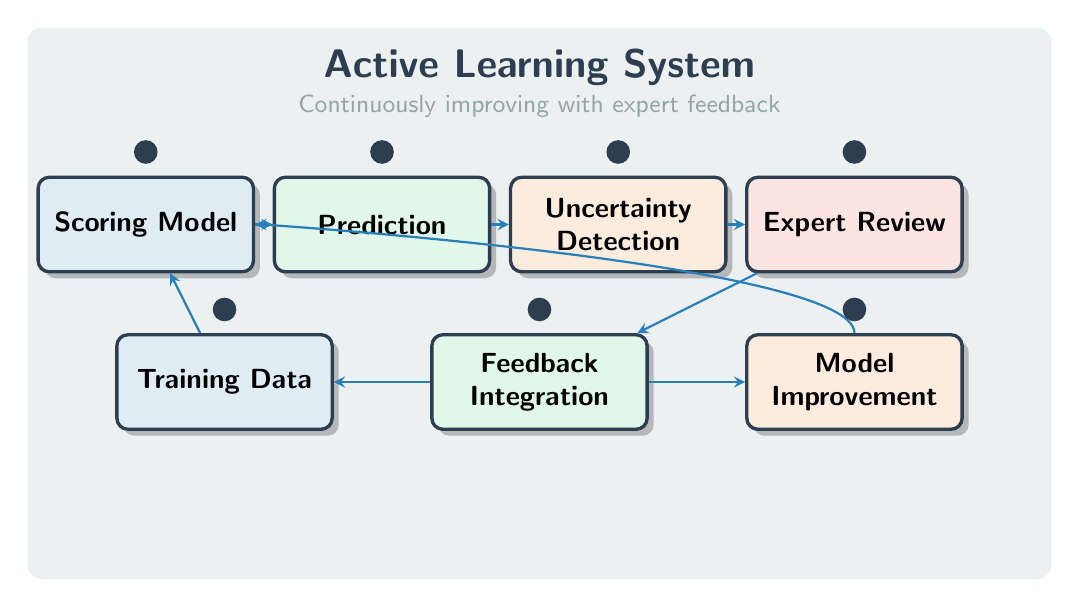
\begin{tikzpicture}[
    node distance=2cm,
    block/.style={
        rectangle,
        rounded corners,
        draw=devtrackdarkblue,
        fill=white,
        very thick,
        text width=2.5cm,
        minimum height=1.2cm,
        text centered,
        font=\sffamily\bfseries,
        drop shadow
    },
    arrow/.style={
        ->,
        >=stealth,
        thick,
        devtrackblue
    },
    title/.style={
        font=\sffamily\bfseries\Large,
        text=devtrackdarkblue
    },
    subtitle/.style={
        font=\sffamily\small,
        text=devtrackgray
    }
]

% Background rectangle
\fill[devtrackbg, rounded corners=5pt] (-0.5,-0.5) rectangle (12.5,6.5);

% Title
\node[title] at (6,6) {Active Learning System};
\node[subtitle] at (6,5.5) {Continuously improving with expert feedback};

% Nodes
\node[block, fill=devtrackblue!15] (model) at (1,4) {Scoring Model};
\node[block, fill=devtrackgreen!15] (predict) at (4,4) {Prediction};
\node[block, fill=devtrackorange!15] (uncertain) at (7,4) {Uncertainty Detection};
\node[block, fill=devtrackred!15] (expert) at (10,4) {Expert Review};

\node[block, fill=devtrackblue!15] (data) at (2,2) {Training Data};
\node[block, fill=devtrackgreen!15] (feedback) at (6,2) {Feedback Integration};
\node[block, fill=devtrackorange!15] (improved) at (10,2) {Model Improvement};

% Arrows
\draw[arrow] (model) -- (predict);
\draw[arrow] (predict) -- (uncertain);
\draw[arrow] (uncertain) -- (expert);
\draw[arrow] (expert) -- (feedback);
\draw[arrow] (data) -- (model);
\draw[arrow] (feedback) -- (data);
\draw[arrow] (feedback) -- (improved);
\draw[arrow] (improved) .. controls +(up:1.5) and +(right:1.5) .. (model);

% Icons
\foreach \pos in {model, predict, uncertain, expert, data, feedback, improved} {
    \fill[devtrackdarkblue] (\pos.north) + (0,0.3) circle (0.15);
}

\end{tikzpicture}

%%%%%%%%%%%%%%%%%%%%%%%%%%%%%%%%%%%%%%%%%
% R2R System
%%%%%%%%%%%%%%%%%%%%%%%%%%%%%%%%%%%%%%%%%
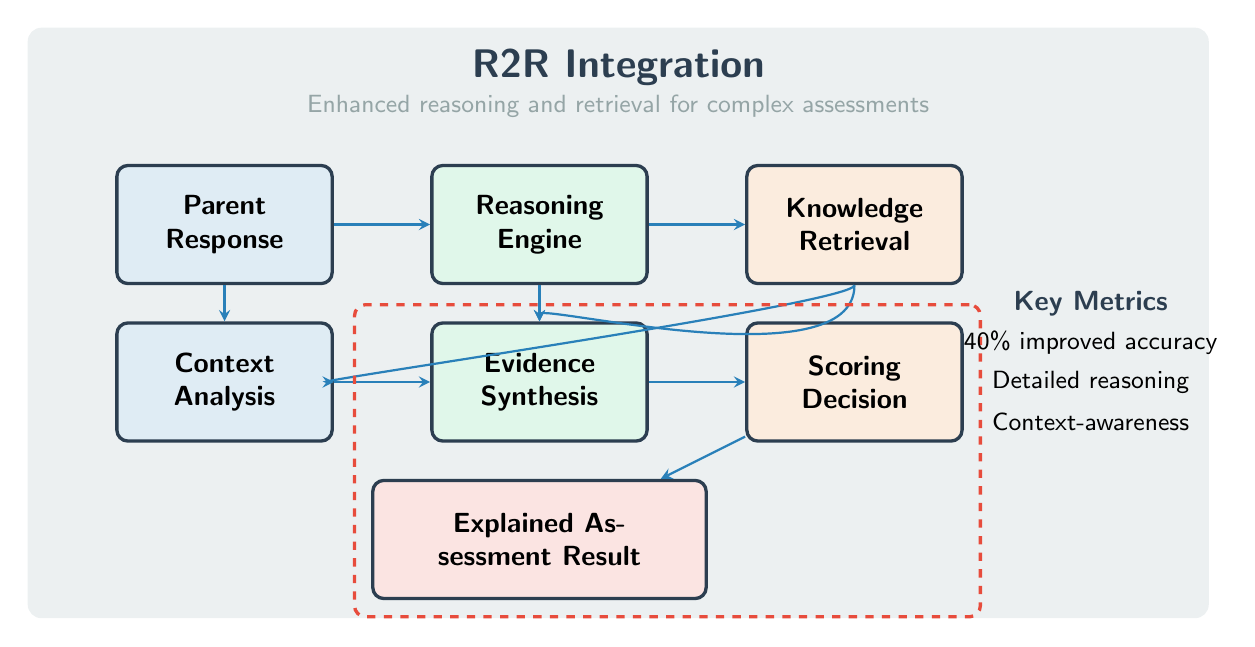
\begin{tikzpicture}[
    node distance=1.5cm,
    block/.style={
        rectangle,
        rounded corners,
        draw=devtrackdarkblue,
        fill=white,
        very thick,
        text width=2.5cm,
        minimum height=1.5cm,
        text centered,
        font=\sffamily\bfseries
    },
    arrow/.style={
        ->,
        >=stealth,
        thick,
        devtrackblue
    },
    title/.style={
        font=\sffamily\bfseries\Large,
        text=devtrackdarkblue
    },
    subtitle/.style={
        font=\sffamily\small,
        text=devtrackgray
    },
    highlight/.style={
        rectangle,
        rounded corners,
        draw=devtrackred,
        dashed,
        very thick,
        inner sep=6pt
    }
]

% Background rectangle
\fill[devtrackbg, rounded corners=5pt] (-0.5,-0.5) rectangle (14.5,7);

% Title
\node[title] at (7,6.5) {R2R Integration};
\node[subtitle] at (7,6) {Enhanced reasoning and retrieval for complex assessments};

% First row
\node[block, fill=devtrackblue!15] (input) at (2,4.5) {Parent Response};
\node[block, fill=devtrackgreen!15] (reason) at (6,4.5) {Reasoning Engine};
\node[block, fill=devtrackorange!15] (retrieve) at (10,4.5) {Knowledge Retrieval};

% Second row
\node[block, fill=devtrackblue!15] (context) at (2,2.5) {Context Analysis};
\node[block, fill=devtrackgreen!15] (synthesis) at (6,2.5) {Evidence Synthesis};
\node[block, fill=devtrackorange!15] (decision) at (10,2.5) {Scoring Decision};

% Output
\node[block, fill=devtrackred!15, text width=4cm] (output) at (6,0.5) {Explained Assessment Result};

% Connections
\draw[arrow] (input) -- (reason);
\draw[arrow] (reason) -- (retrieve);
\draw[arrow] (retrieve) .. controls +(down:1) and +(right:1) .. (context);
\draw[arrow] (input) -- (context);
\draw[arrow] (context) -- (synthesis);
\draw[arrow] (synthesis) -- (decision);
\draw[arrow] (decision) -- (output);
\draw[arrow] (retrieve) .. controls +(down:2) and +(up:1) .. (synthesis);
\draw[arrow] (reason) .. controls +(down:1.5) and +(up:1) .. (synthesis);

% Results highlight
\node[highlight, fit=(decision) (output)] {};

% Key metrics
\node[font=\sffamily\bfseries, text=devtrackdarkblue] at (13,3.5) {Key Metrics};
\node[font=\sffamily\small] at (13,3) {40\% improved accuracy};
\node[font=\sffamily\small] at (13,2.5) {Detailed reasoning};
\node[font=\sffamily\small] at (13,2) {Context-awareness};

\end{tikzpicture}

\end{document} 